\chapterimage{orange2.jpg} % Chapter heading image
\chapterspaceabove{6.75cm} % Whitespace from the top of the page to the chapter title on chapter pages
\chapterspacebelow{7.25cm} % Amount of vertical whitespace from the top margin to the start of the text on chapter pages

\chapter{Lyapunov Stability I: Autonomous Systems}\index{Introduction}

\section{Overview}\index{Overview}
In this chapter, we introduce the concept of Lyapunov stability for autonomous systems. The main objective is to analyze the qualitative behavior of dynamical systems without explicitly solving the differential equations. Lyapunov’s direct method provides a systematic way to assess the stability of equilibrium points by constructing an energy-like function, called a Lyapunov function. 
This approach is particularly powerful because it applies to nonlinear systems where exact solutions are often difficult or impossible to obtain. We also discuss different notions of stability such as stability in the sense of Lyapunov, asymptotic stability, and global stability, laying the foundation for further analysis of nonlinear control systems.

\section{Basic Definitions}\index{Basic Definitions}

Consider the autonomous system
\begin{equation}
    \dot{x} = f(x), \quad x \in \mathbb{R}^n,
\end{equation}
with an equilibrium point $x_e$ such that $f(x_e) = 0$.

\begin{definition}[Stability]
The equilibrium point $x_e$ is said to be \textbf{stable in the sense of Lyapunov} if for every $\varepsilon > 0$, there exists a $\delta > 0$ such that
\[
    \|x(0) - x_e\| < \delta \quad \Rightarrow \quad \|x(t) - x_e\| < \varepsilon, \ \forall t \geq 0.
\]
\end{definition}

\begin{definition}[Convergence]
The equilibrium point $x_e$ is said to be \textbf{convergent} if
\[
    \lim_{t \to \infty} \|x(t) - x_e\| = 0.
\]
\end{definition}

\begin{definition}[Asymptotic Stability]
The equilibrium point $x_e$ is said to be \textbf{asymptotically stable} if it is both stable (in the sense of Lyapunov) and convergent. That is,
\[
    \|x(0) - x_e\| < \delta \quad \Rightarrow \quad 
    \lim_{t \to \infty} \|x(t) - x_e\| = 0.
\]
\end{definition}

\begin{definition}[Exponential Stability]
The equilibrium point $x_e$ is said to be \textbf{exponentially stable} if there exist constants $c > 0$, $\alpha > 0$, and $\delta > 0$ such that
\[
    \|x(0) - x_e\| < \delta \quad \Rightarrow \quad 
    \|x(t) - x_e\| \leq c \, e^{-\alpha t} \, \|x(0) - x_e\|, \quad \forall t \geq 0.
\]
\end{definition}

%---------------------------------------
\section{Geometric Illustration of Stability}

\begin{figure}[h!]
    \centering
    
    % Circle radii (consistent across all subfigures)
    \def\epsrad{1.5}
    \def\deltarad{0.7}
    
    %---------------- (a) Stability ----------------
    \begin{subfigure}[b]{0.45\textwidth}
    \centering
    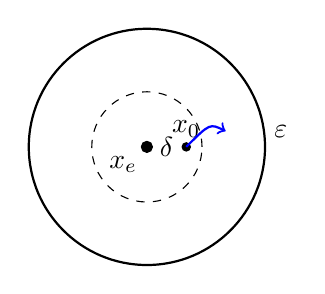
\begin{tikzpicture}[scale=1.0]
        % epsilon circle
        \draw[thick] (0,0) circle (\epsrad);
        \node at (\epsrad+0.2,0.2) {$\varepsilon$};
        % delta circle
        \draw[dashed] (0,0) circle (\deltarad);
        \node at (0.25,0.0) {$\delta$};
        % equilibrium
        \filldraw[black] (0,0) circle (2pt) node[below left] {$x_e$};
        % initial point x0
        \filldraw[black] (0.5,0.0) circle (1.5pt) node[above] {$x_0$};
        % trajectory: stays within epsilon
        \draw[->,blue,thick] (0.5,0.0) .. controls (0.8,0.3) .. (1.0,0.2);
    \end{tikzpicture}
    \caption{Stable: perturbation remains inside $\varepsilon$}
    \end{subfigure}
    \hfill
    %---------------- (b) Convergent ----------------
    \begin{subfigure}[b]{0.45\textwidth}
    \centering
    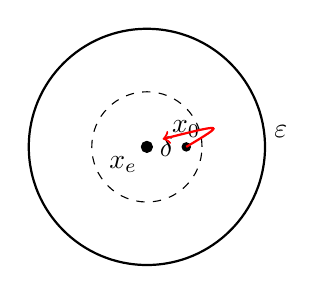
\begin{tikzpicture}[scale=1.0]
        % epsilon circle
        \draw[thick] (0,0) circle (\epsrad);
        \node at (\epsrad+0.2,0.2) {$\varepsilon$};
        % delta circle
        \draw[dashed] (0,0) circle (\deltarad);
        \node at (0.25,0.0) {$\delta$};
        % equilibrium
        \filldraw[black] (0,0) circle (2pt) node[below left] {$x_e$};
        % initial point x0
        \filldraw[black] (0.5,0.0) circle (1.5pt) node[above] {$x_0$};
        % trajectory: moves outward then comes back
        \draw[->,red,thick] (0.5,0.0) .. controls (1.0,0.3) .. (0.2,0.1);
    \end{tikzpicture}
    \caption{Convergent: trajectories return to $x_e$}
    \end{subfigure}
    
    \vspace{0.8cm}
    
    %---------------- (c) Asymptotic stability ----------------
    \begin{subfigure}[b]{0.45\textwidth}
    \centering
    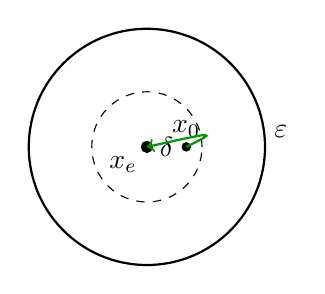
\begin{tikzpicture}[scale=1.0]
        % epsilon circle
        \draw[thick] (0,0) circle (\epsrad);
        \node at (\epsrad+0.2,0.2) {$\varepsilon$};
        % delta circle
        \draw[dashed] (0,0) circle (\deltarad);
        \node at (0.25,0.0) {$\delta$};
        % equilibrium
        \filldraw[black] (0,0) circle (2pt) node[below left] {$x_e$};
        % initial point x0
        \filldraw[black] (0.5,0.0) circle (1.5pt) node[above] {$x_0$};
        % trajectory: goes slightly outward then converges back
        \draw[->,green!60!black,thick] (0.5,0.0) .. controls (0.9,0.2) .. (0.0,0.0);
    \end{tikzpicture}
    \caption{Asymptotically Stable: stable + convergent}
    \end{subfigure}
    \hfill
    %---------------- (d) Exponential stability ----------------
    \begin{subfigure}[b]{0.45\textwidth}
    \centering
    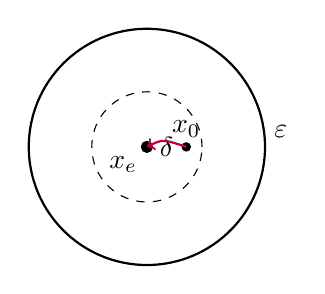
\begin{tikzpicture}[scale=1.0]
        % epsilon circle
        \draw[thick] (0,0) circle (\epsrad);
        \node at (\epsrad+0.2,0.2) {$\varepsilon$};
        % delta circle
        \draw[dashed] (0,0) circle (\deltarad);
        \node at (0.25,0.0) {$\delta$};
        % equilibrium
        \filldraw[black] (0,0) circle (2pt) node[below left] {$x_e$};
        % initial point x0
        \filldraw[black] (0.5,0.0) circle (1.5pt) node[above] {$x_0$};
        % trajectory: sharp fast decay to equilibrium
        \draw[->,purple,thick] (0.5,0.0) .. controls (0.2,0.1) .. (0.0,0.0);
    \end{tikzpicture}
    \caption{Exponentially Stable: fast decay $\sim e^{-\alpha t}$}
    \end{subfigure}

    \caption{Illustrations of stability concepts around equilibrium $x_e$: 
    all trajectories start at an initial condition $x_0$ inside the $\delta$-ball 
    and evolve differently depending on the stability type.}
\end{figure}

%------------------------------------------------
\section{Positive Definite Functions}\index{Positive Definite Functions}

Positive definite functions are the basis of Lyapunov stability theory.  
They provide a way to measure the ``energy'' of a system and are crucial for analyzing stability.

\begin{definition}[Positive Semidefinite Function]
A continuous function $V:\mathcal{D}\subset\mathbb{R}^n \to \mathbb{R}$ is said to be
\begin{itemize}
    \item \textbf{Positive semidefinite} if 
    \[
        V(x) \geq 0, \quad \forall x \in \mathcal{D}, \quad V(0) = 0
    \]
    \item \textbf{Positive definite} if 
    \[
        V(x) > 0 \ \forall x \in \mathcal{D}\setminus\{0\}, \quad V(0)=0
    \]
    \item \textbf{Negative semidefinite} if $V(x) \leq 0$ with equality at the origin.
    \item \textbf{Negative definite} if $V(x) < 0$ for all $x \neq 0$ and $V(0)=0$.
\end{itemize}
\end{definition}

\begin{example}[Quadratic Form]
An important class of functions is given by quadratic forms:
\[
    V(x) = x^T Q x, \quad Q = Q^T \in \mathbb{R}^{n\times n}.
\]
Here,
\begin{itemize}
    \item If $Q$ is positive definite, then $V(x)$ is positive definite.
    \item If $Q$ is positive semidefinite, then $V(x)$ is positive semidefinite.
\end{itemize}
\end{example}

\begin{definition}[Lie Derivative]
Consider a dynamical system 
\[
    \dot{x} = f(x), \quad f:\mathcal{D}\subset\mathbb{R}^n \to \mathbb{R}^n.
\]
For a differentiable function $V:\mathcal{D}\to \mathbb{R}$, the \textbf{Lie derivative} of $V$ along $f$ is defined as
\[
    \dot{V}(x) = L_f V(x) = \nabla V(x)\cdot f(x) =\frac{\partial V}{\partial x}f(x)
\]
\end{definition}

\begin{example}[Computation of $\dot V(x)$]
Consider the nonlinear system
\[
    \dot{x}_1 = 2x_1, 
    \qquad 
    \dot{x}_2 = x_1x_2,
\]
with state vector $x = \begin{bmatrix}x_1 \\ x_2\end{bmatrix}$.

Let the candidate Lyapunov function be
\[
    V(x) = x_1^2 + x_2^2.
\]

Then the gradient of $V$ is
\[
    \nabla V(x) = \begin{bmatrix} 2x_1 & 2x_2 \end{bmatrix}.
\]

Hence the Lie derivative of $V$ along $f(x)$ is
\[
    \dot{V}(x) = \nabla V(x)\cdot f(x) 
    = \begin{bmatrix} 2x_1 & 2x_2 \end{bmatrix}
      \begin{bmatrix} 2x_1 \\ x_1x_2 \end{bmatrix}.
\]

Carrying out the multiplication,
\[
    \dot{V}(x) = 4x_1^2 + 2x_1x_2^2.
\]

\end{example}

\begin{remark}
The sign of $\dot{V}(x)$ (negative definite, semidefinite, or indefinite) determines whether the function $V$ can be used as a Lyapunov function to prove stability of the equilibrium at the origin.
\end{remark}

%------------------------------------------------
\section{Stability Theorems}\index{Stability Theorems}

\begin{theorem}[Lyapunov Stability Theorem]
Consider the autonomous system
\[
    \dot{x} = f(x), \qquad f(0)=0,
\]
with equilibrium at the origin.  
Let $V:\mathcal{D}\to \mathbb{R}$ be a continuously differentiable function such that:
\begin{enumerate}
    \item $V(0) = 0$,
    \item $V(x) > 0, \quad \forall x \in \mathcal{D}\setminus\{0\}$ (positive definite),
    \item $\dot V(x) = \nabla V(x)\cdot f(x) \leq 0, \quad \forall x \in \mathcal{D}\setminus\{0\}$.
\end{enumerate}
Then the equilibrium at the origin is \textbf{stable}.
\end{theorem}

\begin{theorem}[Asymptotic Stability Theorem]
Under the same setup, suppose:
\begin{enumerate}
    \item $V(0) = 0$,
    \item $V(x) > 0, \quad \forall x \in \mathcal{D}\setminus\{0\}$,
    \item $\dot V(x) < 0, \quad \forall x \in \mathcal{D}\setminus\{0\}$ (negative definite).
\end{enumerate}
Then the equilibrium at the origin is \textbf{asymptotically stable}.
\end{theorem}

\begin{example}[Pendulum without Friction]
Consider the undamped pendulum (schematic shown below):

\begin{center}
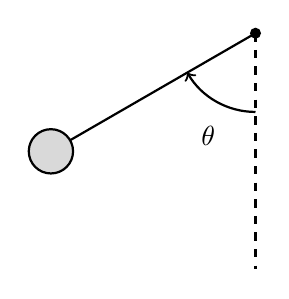
\begin{tikzpicture}[thick,scale=1.0]
    % Pivot point
    \fill (0,0) circle (2pt);

    % String
    \draw (0,0) -- (30:-3);

    % Bob
    \filldraw[fill=gray!30] (30:-3) circle (8pt);

    % Vertical reference line
    \draw[dashed] (0,0) -- (0,-3);

    % Angle theta
    \draw[->] (0,-1) arc (-90:-150:1);
    \node at (-0.6,-1.3) {$\theta$};
\end{tikzpicture}
\end{center}

The dynamics are:
\[
    \ddot{\theta} + \frac{g}{l}\sin\theta = 0.
\]
Define the state variables $x_1 = \theta$, $x_2 = \dot\theta$.  
The system can be written as:
\[
    \dot{x}_1 = x_2, 
    \qquad 
    \dot{x}_2 = -\tfrac{g}{l}\sin(x_1).
\]

Choose the candidate Lyapunov function (total mechanical energy):
\[
    V(x) = \tfrac{1}{2}x_2^2 + \tfrac{g}{l}(1-\cos x_1).
\]

Then
\[
    \dot V(x) = \nabla V(x)\cdot f(x) = x_2\dot{x}_2 + \tfrac{g}{l}\sin(x_1)\dot{x}_1 = 0.
\]

Hence $\dot V(x)=0$, so $V$ is conserved (energy conservation).  
The equilibrium is \textbf{stable}, but not asymptotically stable.
\end{example}


\begin{example}[Pendulum with Friction]
Now consider the damped pendulum:
\[
    \ddot{\theta} + k\dot{\theta} + \tfrac{g}{l}\sin\theta = 0, \quad k>0.
\]
In state-space form:
\[
    \dot{x}_1 = x_2, 
    \qquad 
    \dot{x}_2 = -k x_2 - \tfrac{g}{l}\sin(x_1).
\]

Using the same Lyapunov function:
\[
    V(x) = \tfrac{1}{2}x_2^2 + \tfrac{g}{l}(1-\cos x_1),
\]
we compute
\[
    \dot V(x) = x_2\dot{x}_2 + \tfrac{g}{l}\sin(x_1)\dot{x}_1
    = x_2(-k x_2 - \tfrac{g}{l}\sin(x_1)) + \tfrac{g}{l}\sin(x_1)x_2.
\]

Simplifying,
\[
    \dot V(x) = -k x_2^2 \leq 0,
\]
with equality only when $x_2=0$.  

Thus, $\dot V(x)<0$ for all $x_2 \neq 0$, and the equilibrium is \textbf{asymptotically stable}.
\end{example}

\newpage
%------------------------------------------------
\section{Asymptotic Stability in the Large}\index{Asymptotic Stability in the Large}

\begin{definition}[Global Asymptotic Stability]
	An equilibrium point $x_e$ of $\dot{x}=f(x)$ is said to be \emph{globally asymptotically stable} if it is:
	\begin{enumerate}
		\item Stable in the sense of Lyapunov;
		\item For every initial condition $x(0)\in \mathbb{R}^n$, $\lim_{t\to\infty}x(t)=x_e$.
	\end{enumerate}
\end{definition}

\begin{definition}[Radially Unbounded Function]
	A continuously differentiable function $V:\mathbb{R}^n \to \mathbb{R}$ is said to be \emph{radially unbounded} if
	\begin{equation}
		\|x\| \to \infty \quad \Rightarrow \quad V(x)\to \infty.
	\end{equation}
	In other words, the value of $V(x)$ increases without bound as the norm of $x$ goes to infinity.
\end{definition}

\begin{theorem}[Lyapunov’s Global Stability Theorem]
	Consider the system $\dot{x}=f(x)$ with equilibrium at $x=0$.  
	If there exists a continuously differentiable function $V:\mathbb{R}^n \to \mathbb{R}$ such that:
	\begin{enumerate}
		\item $V(0)=0$,
		\item $V(x)>0$ for all $x\neq 0$,
		\item $V(x)\to \infty$ as $\|x\|\to \infty$ (radially unbounded),
		\item $\dot{V}(x)<0$ for all $x\neq 0$,
	\end{enumerate}
	then the equilibrium $x=0$ is globally asymptotically stable.
\end{theorem}

\begin{example}[Mass–Spring–Damper]
	Consider a mass--spring--damper system:
	\begin{equation}
		m\ddot{x} + c\dot{x} + kx = 0, \quad m,c,k>0.
	\end{equation}
	Choose the Lyapunov function representing the total energy:
	\begin{equation}
		V(x,\dot{x}) = \tfrac{1}{2}m\dot{x}^2 + \tfrac{1}{2}kx^2.
	\end{equation}
	Then:
	\begin{itemize}
		\item $V(x,\dot{x}) \ge 0$, and $V(x,\dot{x}) \to \infty$ as $\|(x,\dot{x})\|\to \infty$ (radially unbounded),
		\item $\dot{V}(x,\dot{x}) = -c\dot{x}^2 < 0$ for $\dot{x}\neq 0$.
	\end{itemize}
	Thus, the equilibrium point $(x,\dot{x})=(0,0)$ is globally asymptotically stable:  
	the mass always comes to rest at the origin, regardless of its initial displacement and velocity.
\end{example}


%------------------------------------------------
\section{Positive Definite Functions Revisited}\index{Positive Definite Functions Revisited}

\begin{definition}[Class $\mathcal{K}$ Functions]
	A continuous function $\alpha:[0,a)\to [0,\infty)$ is said to belong to \emph{class $\mathcal{K}$} if it is:
	\begin{enumerate}
		\item strictly increasing,
		\item $\alpha(0)=0$.
	\end{enumerate}
	If $a=\infty$ and $\alpha(r)\to \infty$ as $r\to \infty$, then $\alpha$ is said to be of \emph{class $\mathcal{K}_\infty$}.
\end{definition}

\begin{corollary}
	A function $V:\mathbb{R}^n \to \mathbb{R}$ is positive definite if and only if there exist class $\mathcal{K}$ functions $\alpha_1, \alpha_2$ such that
	\begin{equation}
		\alpha_1(\|x\|) \leq V(x) \leq \alpha_2(\|x\|), \quad \forall x \in \mathbb{R}^n.
	\end{equation}
\end{corollary}

\begin{corollary}
	Let $x_e$ be an equilibrium of $\dot{x}=f(x)$.  
	If there exists a continuous positive definite function $V(x)$ such that $\dot{V}(x) \leq 0$, then $x_e$ is stable.
\end{corollary}

\begin{corollary}
	Let $x_e$ be an equilibrium of $\dot{x}=f(x)$.  
	If there exists a continuous positive definite function $V(x)$ such that $\dot{V}(x) < 0$ for all $x\neq x_e$, then $x_e$ is asymptotically stable.
\end{corollary}

%------------------------------------------------
\subsection{Exponential Stability}\index{Positive Definite Functions Revisited!Exponential Stability}

\begin{theorem}[Exponential Stability]
	Consider the system $\dot{x}=f(x)$ with equilibrium at $x=0$.  
	If there exists a continuously differentiable, radially unbounded, positive definite function $V(x)$ such that
	\begin{equation}
		c_1 \|x\|^2 \leq V(x) \leq c_2 \|x\|^2,
	\end{equation}
	and
	\begin{equation}
		\dot{V}(x) \leq -c_3 \|x\|^2,
	\end{equation}
	for positive constants $c_1, c_2, c_3 > 0$, then the equilibrium $x=0$ is \emph{globally exponentially stable}.  
	In particular, there exist constants $k,\lambda > 0$ such that
	\begin{equation}
		\|x(t)\| \leq k e^{-\lambda t}\|x(0)\|, \quad \forall t \geq 0.
	\end{equation}
\end{theorem}

\begin{example}[Linear system: global exponential stability]
Consider the system
\begin{equation}
    \dot{x} = Ax,\qquad A=\begin{bmatrix}-1 & 0\\ 0 & -2\end{bmatrix}.
\end{equation}
Choose the Lyapunov function $V(x)=\tfrac{1}{2}\|x\|^2=\tfrac{1}{2}(x_1^2+x_2^2)$. Then
\begin{equation}
    \dot{V}(x) = x^\top \dot{x} = x_1(-x_1)+x_2(-2x_2) = -x_1^2-2x_2^2
    \le -\min\{1,2\}\,(x_1^2+x_2^2) = -\|x\|^2.
\end{equation}
Moreover,
\begin{equation}
    \tfrac{1}{2}\|x\|^2 \le V(x) \le \tfrac{1}{2}\|x\|^2, 
    \qquad \dot{V}(x) \le -\|x\|^2 = -2\,V(x).
\end{equation}
By the exponential stability theorem, $x=0$ is \emph{globally exponentially stable} and
\begin{equation}
    \|x(t)\| \le e^{-t}\|x(0)\|.
\end{equation}
\end{example}

\begin{example}[Nonlinear system: global exponential stability]
Consider the scalar system
\begin{equation}
    \dot{x} = -x - x^3.
\end{equation}
Let $V(x)=\tfrac{1}{2}x^2$. Then
\begin{equation}
    \dot{V}(x) = x\dot{x} = x(-x-x^3) = -x^2 - x^4 \le -x^2 = -2V(x).
\end{equation}
Hence $V$ is positive definite and satisfies $\dot{V}\le -2V$ globally, so the origin is
\emph{globally exponentially stable}. In particular,
\begin{equation}
    |x(t)| \le e^{-t}\,|x(0)|.
\end{equation}
\end{example}

\begin{remark}[Contrast: asymptotic but not exponential]
For the system $\dot{x}=-x^3$ with $V(x)=\tfrac{1}{2}x^2$, we get $\dot{V}=-x^4$.
Although $\dot{V}<0$ for $x\neq 0$ (implying global asymptotic stability), there is no bound of the form
$\dot{V}\le -c\,V$ with a constant $c>0$ valid for all $x$. Thus the origin is \emph{not} exponentially
stable—only (global) asymptotically stable.
\end{remark}

\section{Construction of Lyapunov Functions}\index{Construction of Lyapunov Functions}
\section{The Invariance Principle}\index{The Invariance Principle}
\section{Region of Attraction}\index{Region of Attraction}
\section{Analysis of LTI systems}\index{Analysis of LTI systems}
\section{Instability}\index{Instability}